\documentclass[a4paper,12pt]{article} 
\usepackage[T2A]{fontenc}			
\usepackage[utf8]{inputenc}			
\usepackage[english,russian]{babel}
\usepackage{float}
\usepackage{amsmath,amsfonts,amssymb,amsthm,mathrsfs,mathtools} 
\usepackage{cancel}
\usepackage{multirow}
\usepackage[colorlinks, linkcolor = blue]{hyperref}
\usepackage{upgreek}\usepackage[left=2cm,right=2cm,top=2cm,bottom=3cm,bindingoffset=0cm]{geometry}
\usepackage{tikz}
\usepackage{graphicx}
\usepackage{subfig}
\usepackage{titletoc}
\usepackage{pgfplots}
\usepackage{xcolor}
\usepackage{wrapfig}
\usepackage{pgfplots}
\pgfplotsset{width=10cm,compat=1.9}

\begin{document}

\begin{titlepage}
		\vspace*{\fill}
		
		\begin{center}
			
\includegraphics[scale=0.8]{MIPT.pdf}
			\\[0.7cm]\Huge Московский Физико-Технический Институт
			\\[2cm]\LARGE Отчет по эксперименту
			\\[0.5cm]\noindent\rule{\textwidth}{1pt}
			\\\Huge\textbf{4.7.1. \\ Двойное лучепреломление}
			\\[-0.5cm]\noindent\rule{\textwidth}{1pt}
		\end{center}
		
		\vspace*{\fill}
		
		\begin{flushleft}
			Выполнила: \hspace{\fill} Группа:
			\\Малиновская София \hspace{\fill} Б05-102
		\end{flushleft}
	\end{titlepage}

	\setcounter{page}{2}


\section*{Цель работы}
 Изучение зависимости показателя преломления необыкновенной волны от направления в двоякопреломляющем кристалле; определение главных показателей преломления $n_0$ -- обыкновенной и $n_e$ -- необыкновенной волны в кристалле наблюдение эффекта полного внутреннего отражения.
 
\section*{Оборудование}
Гелий-неоновый лазер, вращающийся столик с неподвижным лимбом, призма из исландского шпата, поляроид.

\section*{Теоретическая сводка}
При падении световой волны на границу изотропной среды в этой среде от границы распространяется одна волна. Если среда анизотропна, то в ней в общем случае возникают две волны -- обыкновенная и необыкновенная, распространяющиеся от границы в разных направлениях и с разными скоростями. При этом связь между вектором напряженности и индукции имеет вид $\textbf{D} = \varepsilon \textbf{E}$, где $\varepsilon$ -- тензор диэлектрической проницаемости. Это явление называется двойным лучепреломлением. \\
Обыкновенный луч ведет себя так же, как и луч в изотропной среде, то есть $n = n_o = \text{const}$. Для необыкновенного луча 
\begin{equation}
    \frac{1}{[n(\theta)]^2} = \frac{\sin^2 \theta}{n_e^2} + \frac{\cos^2 \theta}{n_o^2},
\end{equation}
где $\theta$ -- угол между оптической осью и волновой нормалью, $n_o$ -- показатель преломления волны, распространяющейся вдоль оптической оси, $n_e$ -- показатель преломления волны, распространяющейся перпендикулярно оптической оси. При $n_o - n_e \ll n_o$ формулу (1) можно упростить и представить в виде
\begin{equation}
    n(\theta) \approx n_e + (n_o - n_e)\cos^2 \theta
\end{equation}

\noindent В эксперименте исследуется ход лучей в призме, ход лучей в которой представлен на рис. 1. и рис. 2.

\begin{figure}[H]
    \centering
    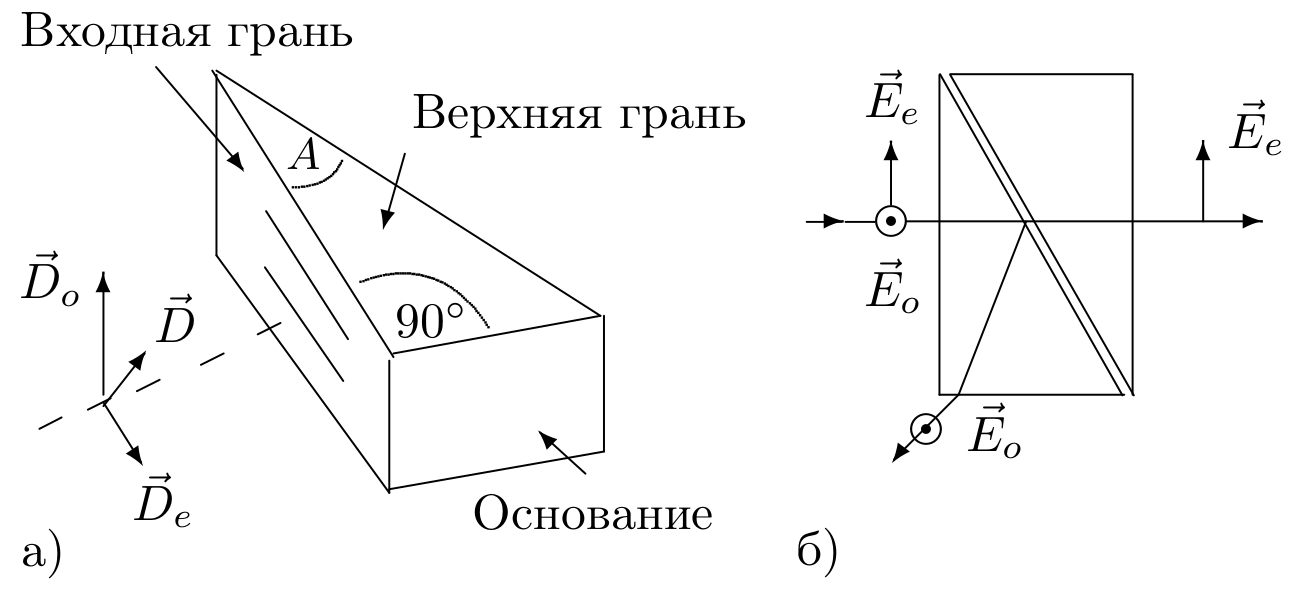
\includegraphics[scale=0.25]{shpat.png}
    \centering
    \caption{а) Исследуемая призма из исландского шпата. б) Ход лучей в поляризационной призме}
\end{figure}

\begin{figure}[H]
    \centering
    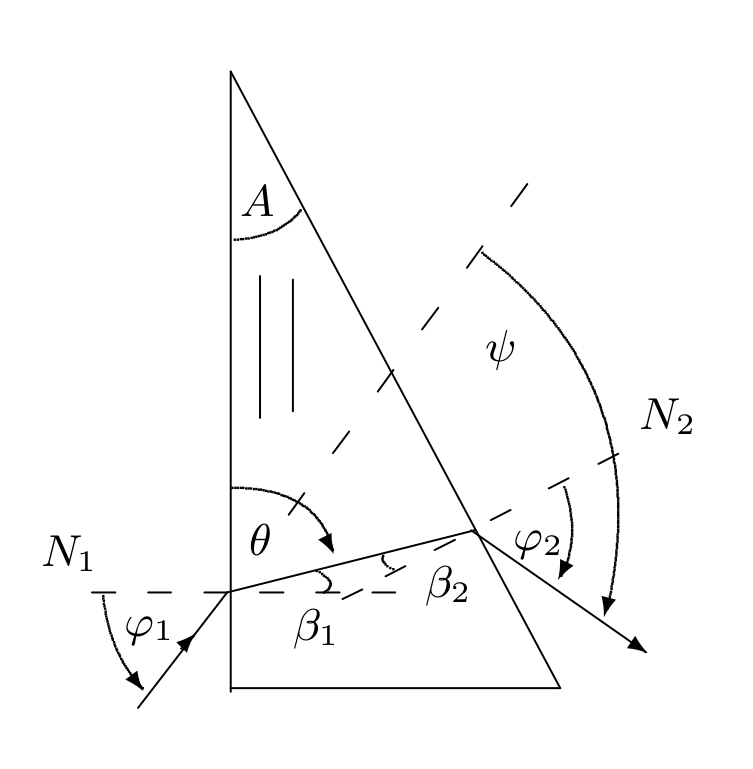
\includegraphics[scale=0.3]{prism.png}
    \caption{Ход лучей в призме}
\end{figure}

\noindent Показатель преломления призмы может быть найден как
\begin{equation}
    n = \frac{1}{\sin A} \sqrt{\sin^2\varphi_1 + \sin^2\varphi_2 + 2\sin\varphi_1\sin\varphi_2\cos A}.
\end{equation}

\noindent Для призмы из изотропного матреиала в случае, когда $\varphi_1 = \varphi_2$, показатель преломления может быть рассчитан по формуле
\begin{equation}
    n = \frac{ \sin\big( \frac{\psi_m + A}{2} \big) }{ \sin\big(\frac{A}{2}\big) },
\end{equation}
где $\psi_m$ -- угол наименьшего отклонения.

\section*{Экспериментальная установка}
\begin{figure}[H]
    \centering
  \begin{minipage}[b]{0.45\textwidth}
    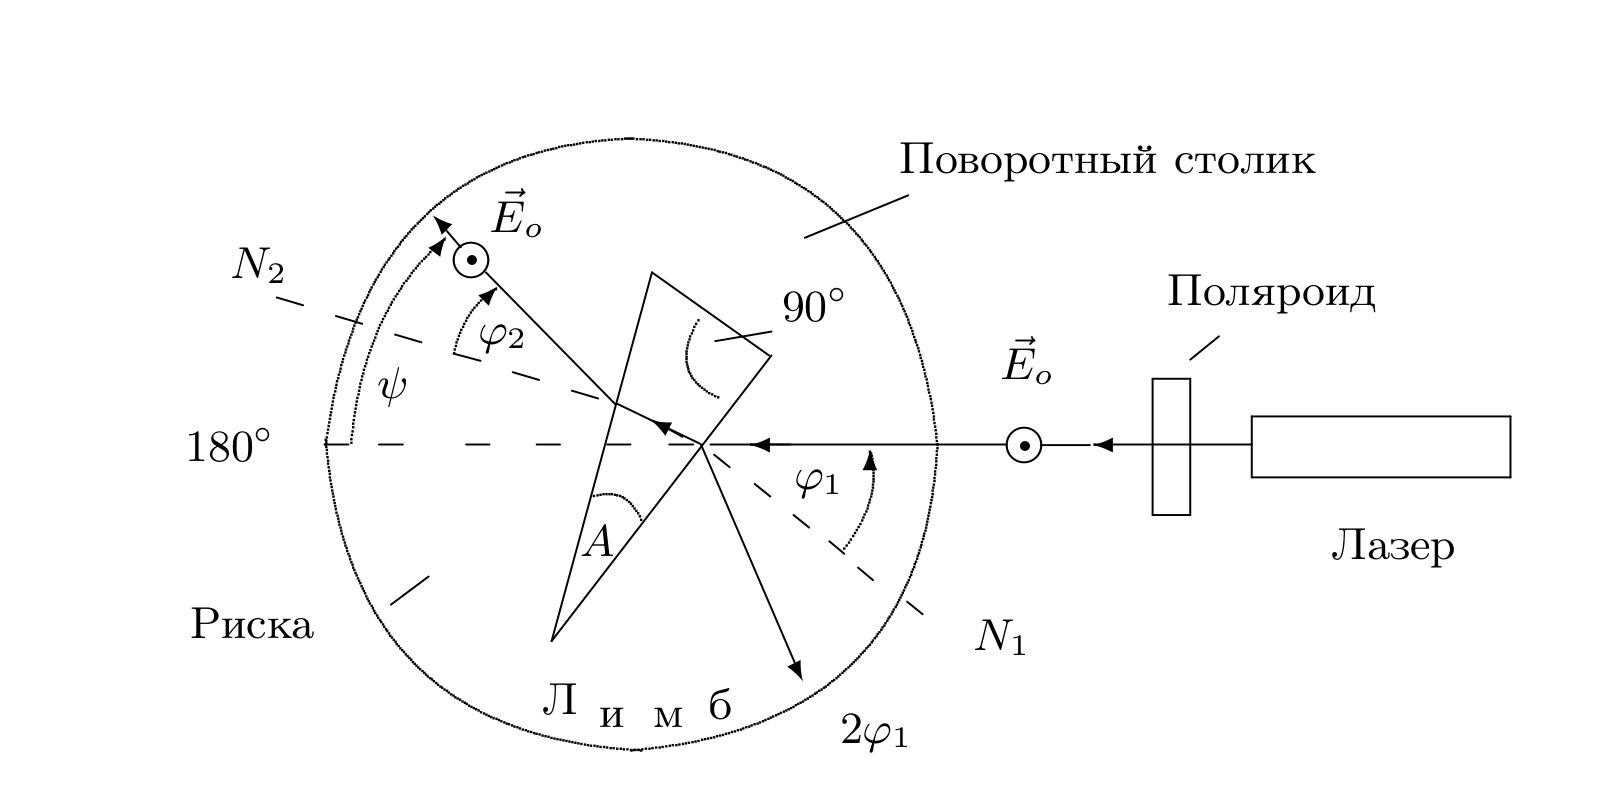
\includegraphics[width=\textwidth]{ust.png}
    \caption{Схема установки}
  \end{minipage}
  \hfill
  \begin{minipage}[b]{0.45\textwidth}
    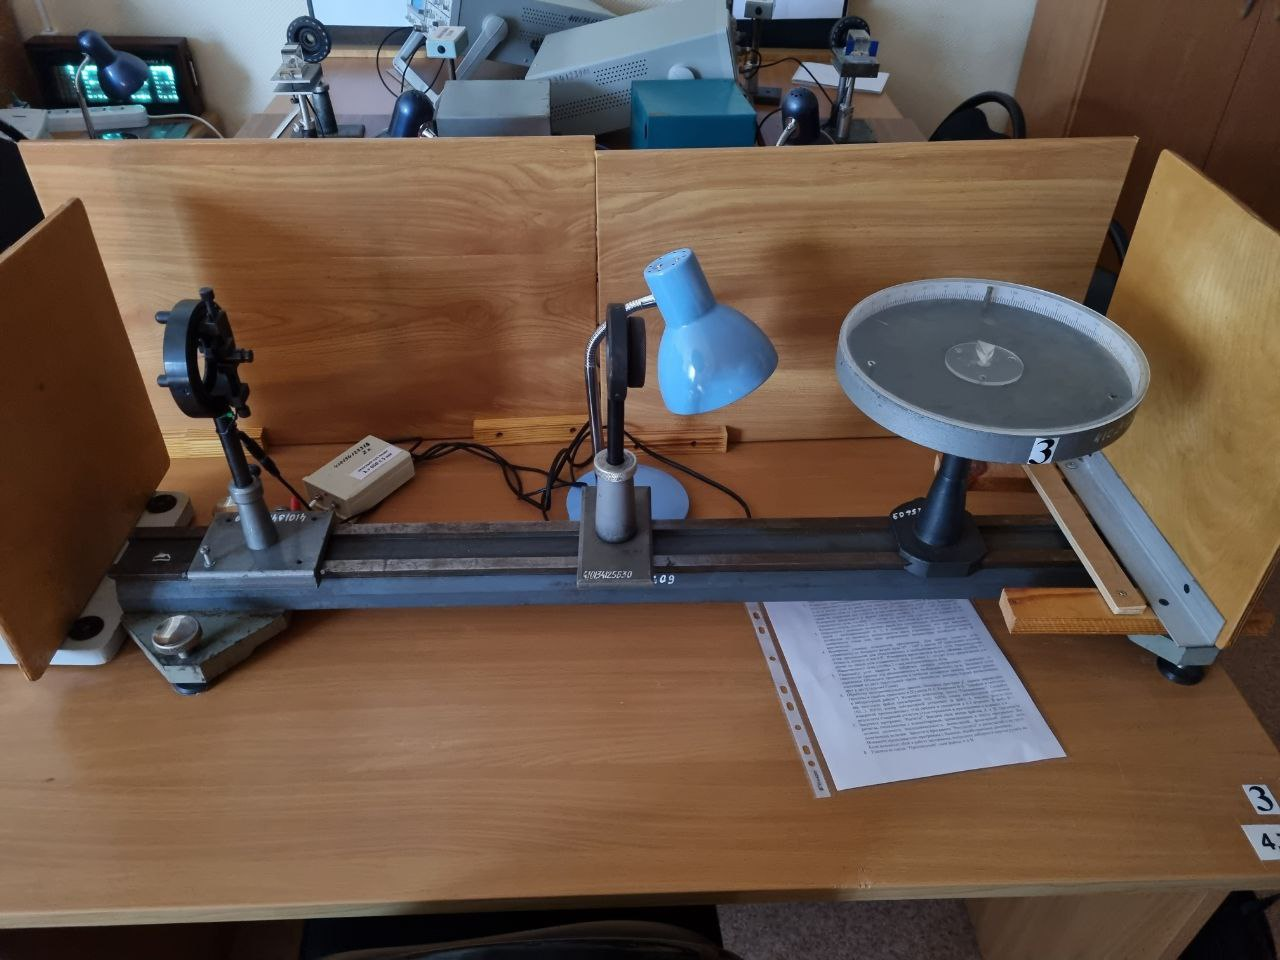
\includegraphics[width=\textwidth]{ex1.jpg}
    \caption{Фотография установки}
  \end{minipage}
\end{figure}

\section*{Ход работы}
Сначала выполним юстировку установки -- столик устанавливим так, чтобы луч проходил через отметки 0 и 180, при этом проходя через центр входного отверстия. \\
Затем определим угол при вершине призмы -- для этого сделаем ряд измерений угла отражения при прохождении луча через катет призмы и гипотенузы призмы. Результаты занесем в таблицу 1. и таблицу 2. Здесь $\alpha$ -- угол, на который был повернут столик.

\begin{table}[H]
\centering
\caption{Преломление луча при прохождении через катет}
\begin{tabular}{|c|c|c|c|c|c|c|c|c|c|c|c|c|c|c|c|}  \hline
$\alpha, ^\circ$ & 0 & 350 & 340 & 330 & 320 & 310 & 300 & 290 & 280 & 270 & 260 & 250 & 240 & 230 & 220 \\ \hline
$2\varphi_1, ^\circ$ & 190 & 185 & 180 & 175 & 170 & 165 & 160 & 155 & 150 & 145 & 140 & 135 & 130 & 125 & 120 \\ \hline
\end{tabular}
\end{table}

\begin{table}[H]
\centering
\caption{Преломление луча при прохождении через гипотенузу}
\begin{tabular}{|c|c|c|c|c|c|c|c|c|c|c|c|c|c|c|c|}  \hline
$\alpha, ^\circ$ & 0 & 350 & 340 & 330 & 320 & 310 & 300 & 290 & 280 & 270 & 260 & 250 & 240 & 230 & 220 \\ \hline
$2\varphi_2, ^\circ$ & 48 & 43 & 38 & 33 & 28 & 23 & 18 & 13 & 8 & 3 & 358 & 353 & 348 & 343 & 338 \\ \hline
\end{tabular}
\end{table}

\noindent По данным из таблицы 2. и таблицы 3. определим угол при вершине призмы $A$
$$
A = 38^\circ\pm0.5^\circ
$$
Затем определим разрешенное направление поляроида, используя для этого стол. Поляриоид нам потребуется для того, чтобы выделять обыкновенную и необыкновенную волны, которые имеют различную поляризацию. \\
Далее снимем зависимость углов отклонения на выходе из призмы для обыкновенной и необыкновенной волны от угла падения луча на призму. Результаты этих измерений представлены в таблице 3.

\begin{table}[H]
    \centering
    \caption{Зависимость углов отклонения от угла падения}
    \begin{tabular}{|c|c|c|} \hline
        $2\varphi, ^\circ$ & $(180 + \psi_o), ^\circ$ & $(180 + \psi_e), ^\circ$ \\ \hline
        20 & 215.5 & 205.5 \\ \hline
        30 & 213.0 & 204.5 \\ \hline
        40 & 211.5 & 204.0 \\ \hline
        50 & 211.0 & 204.0 \\ \hline
        60 & 210.5 & 204.5 \\ \hline
        70 & 211.0 & 205.0 \\ \hline
        80 & 211.5 & 206.0 \\ \hline
        90 & 212.5 & 207.5 \\ \hline
        100 & 214.0 & 209.0 \\ \hline
        110 & 216.0 & 211.5 \\ \hline
        120 & 218.5 & 214.0 \\ \hline
        130 & 222.0 & 216.5 \\ \hline
        140 & 225.0 & 220.0 \\ \hline
    \end{tabular}
\end{table}

\newpage
\noindent Из таблицы 3 также видим, что минимальные значение $\psi_o = 30.5^\circ$, минимальное значение $\psi_e = 24.0^\circ$. По этим величинам проведем вычисления показателся преломления, используя формулу (4)
$$
n_o = 1.673 \pm 0.014
$$
$$
n_e = 1.489 \pm 0.013
$$
\noindent Теперь, использую таблицу 3 рассчитаем значения главного коэффициентов преломления $n_o$ для обыкновенной и $n_e$ для необыкновенной волны, а также величину $\cos^2\theta$. Результаты представлены в таблице 4. Затем потсроим график зависимости $n(\cos\theta)$. Этот график представлен на рис. 5.

\begin{table}[H]
    \centering
    \caption{Вычисленные значения коэффициентов преломления}
    \begin{tabular}{|c|c|c|c|c|c|} \hline
    $\varphi_1, ^\circ$ & $\psi_o, ^\circ$ & $n_o$ & $\psi_e, ^\circ$ & $n_e$ & $\cos^2\theta$ \\ \hline
10.0 & 35.5 & $1.602 \pm 0.011$ & 25.5 & $1.468 \pm 0.011$ & 0.014 \\ \hline
15.0 & 33.0 & $1.597 \pm 0.011$ & 24.5 & $1.472 \pm 0.012$ & 0.031 \\ \hline
20.0 & 31.5 & $1.593 \pm 0.012$ & 24.0 & $1.478 \pm 0.012$ & 0.054 \\ \hline
25.0 & 31.0 & $1.598 \pm 0.012$ & 24.0 & $1.487 \pm 0.012$ & 0.081 \\ \hline
30.0 & 30.5 & $1.593 \pm 0.012$ & 24.5 & $1.501 \pm 0.012$ & 0.111 \\ \hline
35.0 & 31.0 & $1.603 \pm 0.012$ & 25.0 & $1.508 \pm 0.012$ & 0.145 \\ \hline
40.0 & 31.5 & $1.605 \pm 0.012$ & 26.0 & $1.521 \pm 0.012$ & 0.179 \\ \hline
45.0 & 32.5 & $1.611 \pm 0.012$ & 27.5 & $1.538 \pm 0.012$ & 0.211 \\ \hline
50.0 & 34.0 & $1.621 \pm 0.011$ & 29.0 & $1.549 \pm 0.011$ & 0.245 \\ \hline
55.0 & 36.0 & $1.634 \pm 0.011$ & 31.5 & $1.574 \pm 0.011$ & 0.271 \\ \hline
60.0 & 38.5 & $1.650 \pm 0.010$ & 34.0 & $1.591 \pm 0.010$ & 0.296 \\ \hline
65.0 & 42.0 & $1.680 \pm 0.010$ & 36.5 & $1.598 \pm 0.010$ & 0.322 \\ \hline
70.0 & 45.0 & $1.687 \pm 0.010$ & 40.0 & $1.617 \pm 0.009$ & 0.338 \\ \hline
    \end{tabular}
\end{table}

\begin{figure}[H]
    \centering
    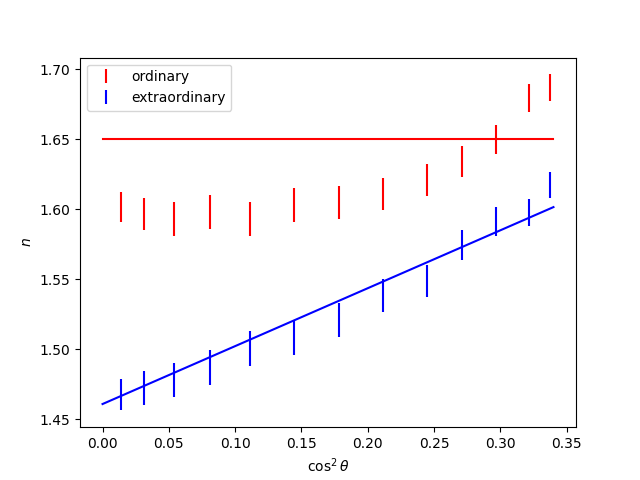
\includegraphics[scale=0.7]{plot.png}
    \caption{Зависимость коэффициента преломления от квадрата косинуса}
\end{figure}

\noindent Видим, что для необыкновенной волны выполняется соотношение (2), а для обыкновенной также заметно изменение от угла. Окончательные значения главных коэффициентов преломления найдем как среднее арифметическое соответствующих величин
$$
n_o = 1.649 \pm 0.008
$$
$$
n_e = 1.502 \pm 0.008
$$

\noindent Наконец, добьемся полного внутреннего отражения каждого из лучей, и с помощью него определим коэффициенты преломления. Полное внутренне отражение обыкновенной волны достигается при $2\varphi = 2^\circ\pm2^\circ$, а необыкновенной -- при $2\varphi = 8^\circ\pm3^\circ$. Отсюда
$$
n_o = 1.661\pm0.038
$$
$$
n_e = 1.494\pm0.043
$$

\section*{Вывод}
В работе были изучена зависимость показателся преломления необыкновенной волны от направления ее распространения в двоякопреломляющем кристалле. Несколькими способами были определены значения главных показателей преломления обыкновенной и необыкновенной волны. 
\begin{itemize}
    \item При измерении по минимальному углу получены значения $n_o = 1.673 \pm 0.014$, $n_e = 1.489 \pm 0.013$
    \item При измерении множества коэффициентов преломления при различных углах и последующем усреднении получены значения $n_o = 1.649 \pm 0.008$, $n_e = 1.502 \pm 0.008$
    \item При измерении по углу полного внутреннего отражения получены значения $n_o = 1.661\pm0.038$, $n_e = 1.494\pm0.043$
\end{itemize}
Табличные значения этой величины для кальцита, разновидностью которого является исландский шпат, составляют $n_o = 1.640 \textit{ --- } 1.660$, $n_e = 1.486$. \\
\noindent То что получены близкие между собой и к теории, но различные в пределах погрешности величины, объясняется тем, что при измерениях использовался поляроид, настраиваемый по отражению от плоскости стола, в результате чего разрешенное направление поляроида могло быть установлено не вертикально, а под небольшим углом к горизонту, в результате чего необыкновенная волна оказывала влияние на измерения для обыкновенной, и наоборот. Также стоит отметить, что измерения по углу полного внутреннего отражения являются приблизительными, так как при достижении полного внутреннего отражения преломленный луч не исчезает сразу, а постепенно теряет яркость, из-за чего можно измерить лишь интревал, в котором достигается полное внутреннее отражение.

\end{document}

